\documentclass[11pt, a4paper]{article}
%\usepackage{proj1}
\usepackage{natbib}
\usepackage{fancyhdr}  
\usepackage{subcaption}
\usepackage{caption}
\usepackage{graphicx}
\usepackage{numprint}
\usepackage{multirow}
\linespread{1.25} 
\setlength{\parindent}{0cm}
\graphicspath{{Images/}}
\usepackage{hyperref}
\usepackage{amsmath}
\usepackage{amsfonts}
\usepackage{amssymb}
\usepackage{amsthm}
\usepackage{mathtools}
\usepackage{commath}
\usepackage{bbm}

%\usepackage[sc,osf]{mathpazo}
\usepackage{subcaption}
\usepackage[a4paper, top=1in, left=1.0in, right=1.0in, bottom=1in, includehead, includefoot]{geometry} %Usually have top as 1in

\usepackage{listings}
\usepackage{color} %red, green, blue, yellow, cyan, magenta, black, white
\definecolor{mygreen}{RGB}{28,172,0} % color values Red, Green, Blue
\definecolor{mylilas}{RGB}{170,55,241}


\hypersetup{colorlinks,linkcolor={black},citecolor={blue},urlcolor={black}}
\usepackage{color}
\urlstyle{same}


\theoremstyle{definition}
\newtheorem{definition}{Definition}[section]

\newcommand{\adja}{q_a}
\newcommand{\adjb}{q_b}
\newcommand{\adjaB}{q_{a,\partial \Omega}}
\newcommand{\adjbB}{q_{b,\partial \Omega}}
\newcommand{\adjB}{q_{\partial \Omega}}
\newcommand{\Adja}{\mathbf{p}}
\newcommand{\Adjb}{q}
\newcommand{\adj}{q}
\newcommand{\Adjc}{{q}_{\partial \Omega}}
\newcommand{\ra}{\rho_a}
\newcommand{\rb}{\rho_b}
\newcommand{\w}{\mathbf{w}}
\newcommand{\f}{\mathbf{f}}
\newcommand{\ve}{\mathbf{v}}
\newcommand{\n}{\mathbf{n}}
\newcommand{\h}{\mathbf{h}}
\newcommand{\K}{\mathbf{K}}
\newcommand{\hr}{\widehat \rho}
\newcommand{\jf}{\mathbf j}

%	\begin{figure}[h]
%		\centering
%		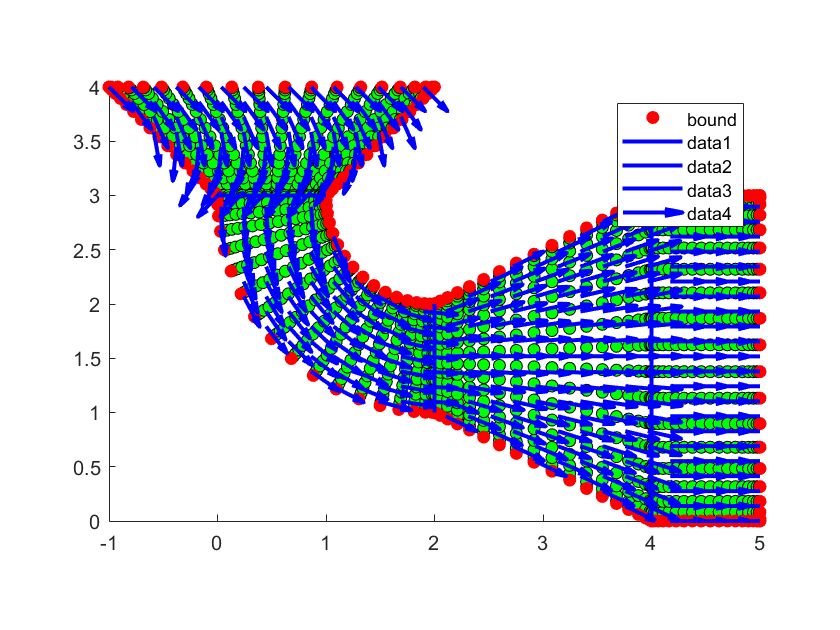
\includegraphics[scale=0.35]{F1.png}
%		\caption{Forward $\rho$ for $a = 0.01$} 
%		\label{F1}
%	\end{figure}

\begin{document}
\section*{MultiShape Theory ++++ go to ShapeNotes}

\section{Validation Tests}


\subsection{Testing Differentiation, Interpolation, Convolution and Integration}
We investigate the accuracy of the different operations in the following way.
The differentiation matrix is compared against the exact solution
\begin{align*}
	\rho &= \exp( \alpha_1  t + \beta_1 y_1 + \beta_2 y_2),\\
	\nabla \rho &= [\beta_1 \rho, \beta_2 \rho],\\
	\nabla^2 \rho &= \nabla \cdot \nabla \rho = (\beta_1^2 + \beta_2^2)\rho,
\end{align*}
where $	\beta_1 = 0.1 $, $\beta_2 = 0.1$, $\alpha_1 = -0.5$.
In polar coordinates we choose (++++ not right yet +++)
\begin{align*}
	\rho & = r \cos(\theta),\\
	\nabla \rho &= [\cos (\theta), -\sin (\theta)],\\
	\nabla^2 \rho & = \nabla \cdot \nabla \rho = - \sin( \theta).
\end{align*}

We compare each of the operators gradient, divergence and Laplacian against the exact solution, where the divergence test is done by taking the divergence of the exact solution for $\nabla \rho$ and comparing it to the exact solution for $\nabla^2 \rho$. The solutions can be seen in Tables \ref{Tab:Grad}, \ref{Tab:Lap} and \ref{Tab:div}.

\begin{table}
	\caption{Errors against an exact solution for gradient}
	\begin{tabular}{ ||c| c| c| c| c |c|c|| }
		\hline
		\hline
		& A.E. $N =10$ & R.E. $N =10$ &A.E. $N =20$ & R.E. $N =20$ &A.E. $N =30$ & R.E. $N =30$ \\ 
		a& $ 1.5572\times 10^{- 14}$ & $ 1.4701\times 10^{- 14}$ & $2.0596 \times 10^{-13 }$ & $9.7269 \times 10^{-14 }$ &$ 5.7697\times 10^{-13 }$ & $1.8169 \times 10^{-13 }$ \\
		b& $ 6.1347\times 10^{- 14}$ & $4.0407 \times 10^{-14 }$ & $ 5.0572\times 10^{- 13}$ & $ 1.6660\times 10^{- 13}$ &$1.8894 \times 10^{- 12}$ & $ 4.1501\times 10^{- 13}$ \\
		f& $ 1.9073\times 10^{-13 }$ & $ 8.6807\times 10^{-14 }$ & $1.6899 \times 10^{-12 }$ & $ 3.8462\times 10^{- 13}$ &$ 6.2172\times 10^{-12 }$ & $ 9.4338\times 10^{- 13}$ \\
		\hline
		h& $ \times 10^{- }$ & $ \times 10^{- }$ & $ \times 10^{- }$ & $ \times 10^{- }$ &$ \times 10^{- }$ & $ \times 10^{- }$ \\
		j& $ \times 10^{- }$ & $ \times 10^{- }$ & $ \times 10^{- }$ & $ \times 10^{- }$ &$ \times 10^{- }$ & $ \times 10^{- }$ \\
		k& $ \times 10^{- }$ & $ \times 10^{- }$ & $ \times 10^{- }$ & $ \times 10^{- }$ &$ \times 10^{- }$ & $ \times 10^{- }$ \\
		\hline
	\end{tabular}
\label{Tab:Grad}
\end{table}

\begin{table}
	\caption{Errors against an exact solution for Lap}
	\begin{tabular}{ ||c| c| c| c| c |c|c|| }
		\hline
		\hline
		& A.E. $N =10$ & R.E. $N =10$ &A.E. $N =20$ & R.E. $N =20$ &A.E. $N =30$ & R.E. $N =30$ \\ 
		a& $5.0430 \times 10^{- 13}$ & $3.3666 \times 10^{-12 }$ & $1.8696 \times 10^{-11 }$ & $ 6.2434\times 10^{- 11}$ &$ 8.1857\times 10^{- 11}$ & $1.8227 \times 10^{- 10}$ \\
		b& $ 3.6405\times 10^{-12 }$ & $ 1.6955\times 10^{- 11}$ & $ 1.5930\times 10^{-10}$ & $ 3.7109\times 10^{- 10}$ &$ 5.5595\times 10^{-10 }$ & $8.6347 \times 10^{-10 }$ \\
		f& $ 3.2770\times 10^{-11 }$ & $ 1.0546\times 10^{-10 }$ & $ 1.5373\times 10^{-9 }$ & $2.4741 \times 10^{- 9}$ &$ 7.5560\times 10^{- 9}$ & $8.1072 \times 10^{-9 }$ \\
		\hline
		h& $ \times 10^{- }$ & $ \times 10^{- }$ & $ \times 10^{- }$ & $ \times 10^{- }$ &$ \times 10^{- }$ & $ \times 10^{- }$ \\
		j& $ \times 10^{- }$ & $ \times 10^{- }$ & $ \times 10^{- }$ & $ \times 10^{- }$ &$ \times 10^{- }$ & $ \times 10^{- }$ \\
		k& $ \times 10^{- }$ & $ \times 10^{- }$ & $ \times 10^{- }$ & $ \times 10^{- }$ &$ \times 10^{- }$ & $ \times 10^{- }$ \\
		\hline
	\end{tabular}
	\label{Tab:Lap}
\end{table}
\begin{table}
	\caption{Errors against an exact solution for Div}
	\begin{tabular}{ ||c| c| c| c| c |c|c|| }
		\hline
		\hline
		& A.E. $N =10$ & R.E. $N =10$ &A.E. $N =20$ & R.E. $N =20$ &A.E. $N =30$ & R.E. $N =30$ \\ 
		a& $  1.8961\times 10^{- 15}$ & $ 1.2658\times 10^{-14 }$ & $2.1857 \times 10^{- 14}$ & $7.2992 \times 10^{-14 }$ &$6.4880 \times 10^{-14 }$ & $1.4447 \times 10^{- 13}$ \\
		b& $ 6.8661\times 10^{-15}$ & $ 3.1978\times 10^{- 14}$ & $ 5.3498\times 10^{-14 }$ & $ 1.2462\times 10^{-13 }$ &$ 2.0321\times 10^{-13 }$ & $3.1561 \times 10^{-13 }$ \\
		f& $ 2.2352\times 10^{-14 }$ & $ 7.1934\times 10^{-14 }$ & $ 1.6133\times 10^{-13 }$ & $ 2.5964\times 10^{-13 }$ &$5.7670 \times 10^{-13 }$ & $ 6.1877\times 10^{- 13}$ \\
		\hline
		h& $ \times 10^{- }$ & $ \times 10^{- }$ & $ \times 10^{- }$ & $ \times 10^{- }$ &$ \times 10^{- }$ & $ \times 10^{- }$ \\
		j& $ \times 10^{- }$ & $ \times 10^{- }$ & $ \times 10^{- }$ & $ \times 10^{- }$ &$ \times 10^{- }$ & $ \times 10^{- }$ \\
		k& $ \times 10^{- }$ & $ \times 10^{- }$ & $ \times 10^{- }$ & $ \times 10^{- }$ &$ \times 10^{- }$ & $ \times 10^{- }$ \\
		\hline
	\end{tabular}
	\label{Tab:div}
\end{table}

We investigate the functionality of the interpolation matrix by interpolating from shape (a)/ (h) with $N = 50$ onto different shapes with smaller $N$ and compare to the exact solution on the other shapes. The results can be seen in Table \ref{Tab:Interp}.

\begin{table}
	\caption{Interpolation error from shape (a) to (b), (f), (g) and from (h) to (j), (k)}
	\begin{tabular}{ ||c| c| c| c| c |c|c|| }
		\hline
		\hline
		& A.E. $N =10$ & R.E. $N =10$ &A.E. $N =20$ & R.E. $N =20$ &A.E. $N =30$ & R.E. $N =30$ \\ 
		b& $  9.9692\times 10^{- 15}$ & $ 9.3107\times 10^{-15 }$ & $2.2223 \times 10^{- 14}$ & $1.0388 \times 10^{-15 }$ &$ 4.5668 \times 10^{-14 }$ & $1.4236 \times 10^{- 15}$ \\
	    f& $ 1.4603\times 10^{-14}$ & $9.2190 \times 10^{- 16}$ & $4.1259 \times 10^{-14 }$ & $1.3028 \times 10^{-15 }$ &$6.1716 \times 10^{-14 }$ & $1.2993\times 10^{-15 }$ \\
		g& $ 1.6536\times 10^{-14 }$ & $1.0990 \times 10^{-15 }$ & $4.4612 \times 10^{-14 }$ & $ 1.4828\times 10^{-15 }$ &$ 7.0500\times 10^{-14 }$ & $1.5623 \times 10^{- 15}$ \\
		\hline
		j& $1.7639 \times 10^{-14 }$ & $1.0602 \times 10^{- 15}$ & $3.6280 \times 10^{- 14}$ & $ 1.0920\times 10^{- 15}$ &$7.6534 \times 10^{-14 }$ & $ 1.5366\times 10^{- 15}$ \\
		k& $ 1.8849\times 10^{-14 }$ & $9.6282 \times 10^{- 16}$ & $ 6.3049\times 10^{-14 }$ & $ 1.6108\times 10^{- 15}$ &$ 9.2844\times 10^{-14 }$ & $1.5815 \times 10^{- 15}$ \\
		\hline
	\end{tabular}
	\label{Tab:Interp}
\end{table}

We consider the same approach for testing the convolution matrix. We compute the convolution with $N = 50$ on shape (a) (or (h) respectively) and apply it to some function $\rho$. (exact solution above). We then interpolate this onto the other shapes and compute the error with the convolution of $\rho$ on that shape. The results are displayed in Table \ref{Tab:conv}.

For the integration vector, we compute the integral of $\rho$ on shape (a) and compare this to the integral of $\rho$ on shape (b), (f) and (g). We then compare the integral of $\rho$ on (h) to the one on (j) and (k). This can be seen in Table \ref{Tab:int}.


\begin{table}
	\caption{Convolution error from shape (a) to (b), (f), (g) and from (h) to (j), (k)}
	\begin{tabular}{ ||c| c| c| c| c |c|c|| }
		\hline
		\hline
		& A.E. $N =10$ & R.E. $N =10$ &A.E. $N =20$ & R.E. $N =20$ &A.E. $N =30$ & R.E. $N =30$ \\ 
		b& $ 7.2818\times 10^{- 7}$ & $ 4.7687\times 10^{-8}$ & $ 6.2092\times 10^{- 14}$ & $2.0049\times 10^{-15 }$ &$ 1.2357\times 10^{-13 }$ & $2.6477\times 10^{- 15}$ \\
		f& $ 1.2855\times 10^{-7}$ & $ 5.7524\times 10^{- 9}$ & $ 1.1475\times 10^{-13 }$ & $ 2.5524\times 10^{-15 }$ &$ 1.9523\times 10^{-13 }$ & $ 2.8894\times 10^{-15 }$ \\
		g& $ 1.5819 \times 10^{-9 }$ & $ 6.5996\times 10^{-11 }$ & $ 1.1647\times 10^{-13 }$ & $ 2.4210\times 10^{-15 }$ &$ 1.9834\times 10^{-13 }$ & $2.7453 \times 10^{- 15}$ \\
		\hline
		j& $  0.0033$ & $ 1.6340 \times 10^{-4 }$ & $ 2.1798\times 10^{- 7}$ & $5.3326 \times 10^{- 9}$ &$3.7177 \times 10^{- 11}$ & $ 6.0314\times 10^{- 13}$ \\
		k& $ 7.1090\times 10^{-6 }$ & $2.8527 \times 10^{-7 }$ & $ 4.8469\times 10^{- 12}$ & $9.6680\times 10^{-14 }$ &$ 2.1566\times 10^{- 13}$ & $2.8622 \times 10^{- 15}$ \\
		\hline
	\end{tabular}
	\label{Tab:conv}
\end{table}



\begin{table}
	\caption{Integration error from shape (a) to (b), (f), (g) and from (h) to (j), (k)}
	\begin{tabular}{ || c| c| c| c| c| c| c||| }
		\hline
		\hline
		a, $N =50$ & b, $N =10$& f, $N =10$ & g, $N =10$& h, $N =50$& j, $N =10$& k, $N =10$\\ 
		 $ 2.9831$ & $2.9831 $ & $2.9831 $ &$2.9831 $ & $5.3391 $ & $5.3391$ &  $5.3391 $  \\

		\hline
	\end{tabular}
	\label{Tab:int}
\end{table}



\subsection{Exact Tests - Dirichlet Conditions}
(MS\_TestJonnaADExactDisectBoxes and MS\_TestJonnaADExactDisectBoxesPart2 and MS\_TestJonnaADExactDisectWedges)
Several examples are run, using exact solutions, to validate the multishape code. This is done using an exact solution to the advection diffusion equation on an infinite domain, so that Dirichlet boundary conditions, matching the value of the exact solution on the boundary of the multishape, can be applied.
The exact solution is \cite{Hutomo_2019}
\begin{align*}
	\rho &= \exp(\alpha t + \beta_1 y_1 + \beta_2 y_2)\\
	\mathbf v &= \left(\beta_1 - \frac{\alpha}{2 \beta_1} + p_1\exp(-\beta_1 y_1) , \beta_2 - \frac{\alpha}{2 \beta_2} + p_2\exp(-\beta_2 y_2) \right),
\end{align*}
where $\beta_1 = 0.1$, $\beta_2 = 0.1$, $\alpha = -0.5$, $p_1 = -1$ and $p_2 = 1$.
We compare the exact solution on a box of dimensions $[0,2] \times [0,2] $ with different discretizations of the box using multishape, see Figure \ref{F2}. Each of the shapes are discretized with $N = 20$ and $N = 30$ points in each spatial direction, which means that the dissected box has more points in total than the original box. The ODE solver tolerances are $10^{-9}$. The solution can be seen in Figure \ref{F3}. The question is whether the results of the PDE on the box and the different discretizations of the box have a similar error when compared to the exact solution. The absolute and relative errors are measured in an $L_2$ norm in space and an $L_\infty$ norm in time and are displayed in Table \ref{Tab1:ErrorsExBox}. The bottom row contains errors for the non-rectangular quadrilateral, which is shown in Figure \ref{F3a}. 
\begin{table}
	\caption{Errors compared to exact solution for different discretizations of the box and a quadrilateral (absolute error A.E. and relative error R.E. are compared)}
	\begin{tabular}{ ||c| c| c| c| c |c|c|| }
		\hline
		\hline
		& A.E. $N =10$ & R.E. $N =10$ &A.E. $N =20$ & R.E. $N =20$ &A.E. $N =30$ & R.E. $N =30$ \\ 
		\hline
		a & $2.5869 \times 10^{-7}$ & $1.0894 \times 10^{-9}$ & $2.2063 \times 10^{-7}$ & $1.1235 \times 10^{-9}$ & $2.1913 \times 10^{-7}$ & $1.1159 \times 10^{-9}$ \\  
		b & $3.4991\times 10^{-7}$ & $1.1308 \times 10^{-9}$ &  $3.2073 \times 10^{-7}$ & $1.1377 \times 10^{-9}$  & $3.1878 \times 10^{-7}$ & $1.1308 \times 10^{-9}$\\  
		c & $4.1386\times 10^{-7}$  & $1.1596 \times 10^{-9}$ & $3.9108\times 10^{-7}$ & $1.15 \times 10^{-9}$  & $3.8859\times 10^{-7}$ & $1.1427\times 10^{-9}$ \\  
		d & $4.2622\times 10^{-7}$ & $1.0268 \times 10^{-9} $& $3.902\times 10^{-7}$ & $1.0026 \times 10^{-9}$ & $3.8767\times 10^{-7}$ & $9.9612 \times 10^{-10}$\\
		e & $4.1985 \times 10^{-7}$ & $1.0275 \times 10^{-9}$  & $4.2546 \times 10^{-7}$ & $1.0412 \times 10^{-9}$  & $4.2292 \times 10^{-7}$  & $1.035 \times 10^{-9}$ \\
		f & $4.4594 \times 10^{-7}$  & $1.0704 \times 10^{-9}$ & $3.3849 \times 10^{-7}$ & $9.8249 \times 10^{-10}$&  $3.3719 \times 10^{-7}$&  $1.0085 \times 10^{-9}$\\
		g & $5.0161\times 10^{-7}$ & $1.1254 \times 10^{-9}$  & $4.4469\times 10^{-7}$& $1.1323 \times 10^{-9}$ &  $4.3978\times 10^{-7}$& $1.1198\times 10^{-9}$\\
		q & $2.4145\times 10^{-7}$ & $1.0389\times 10^{-9}$ & $2.2844\times 10^{-7}$ & $1.116\times 10^{-9}$ & $2.2505\times 10^{-7}$ & $1.0995\times 10^{-9}$\\
		\hline
		\hline
	\end{tabular}
	\label{Tab1:Errors}
\end{table}
	\begin{figure}[h]
		\centering
		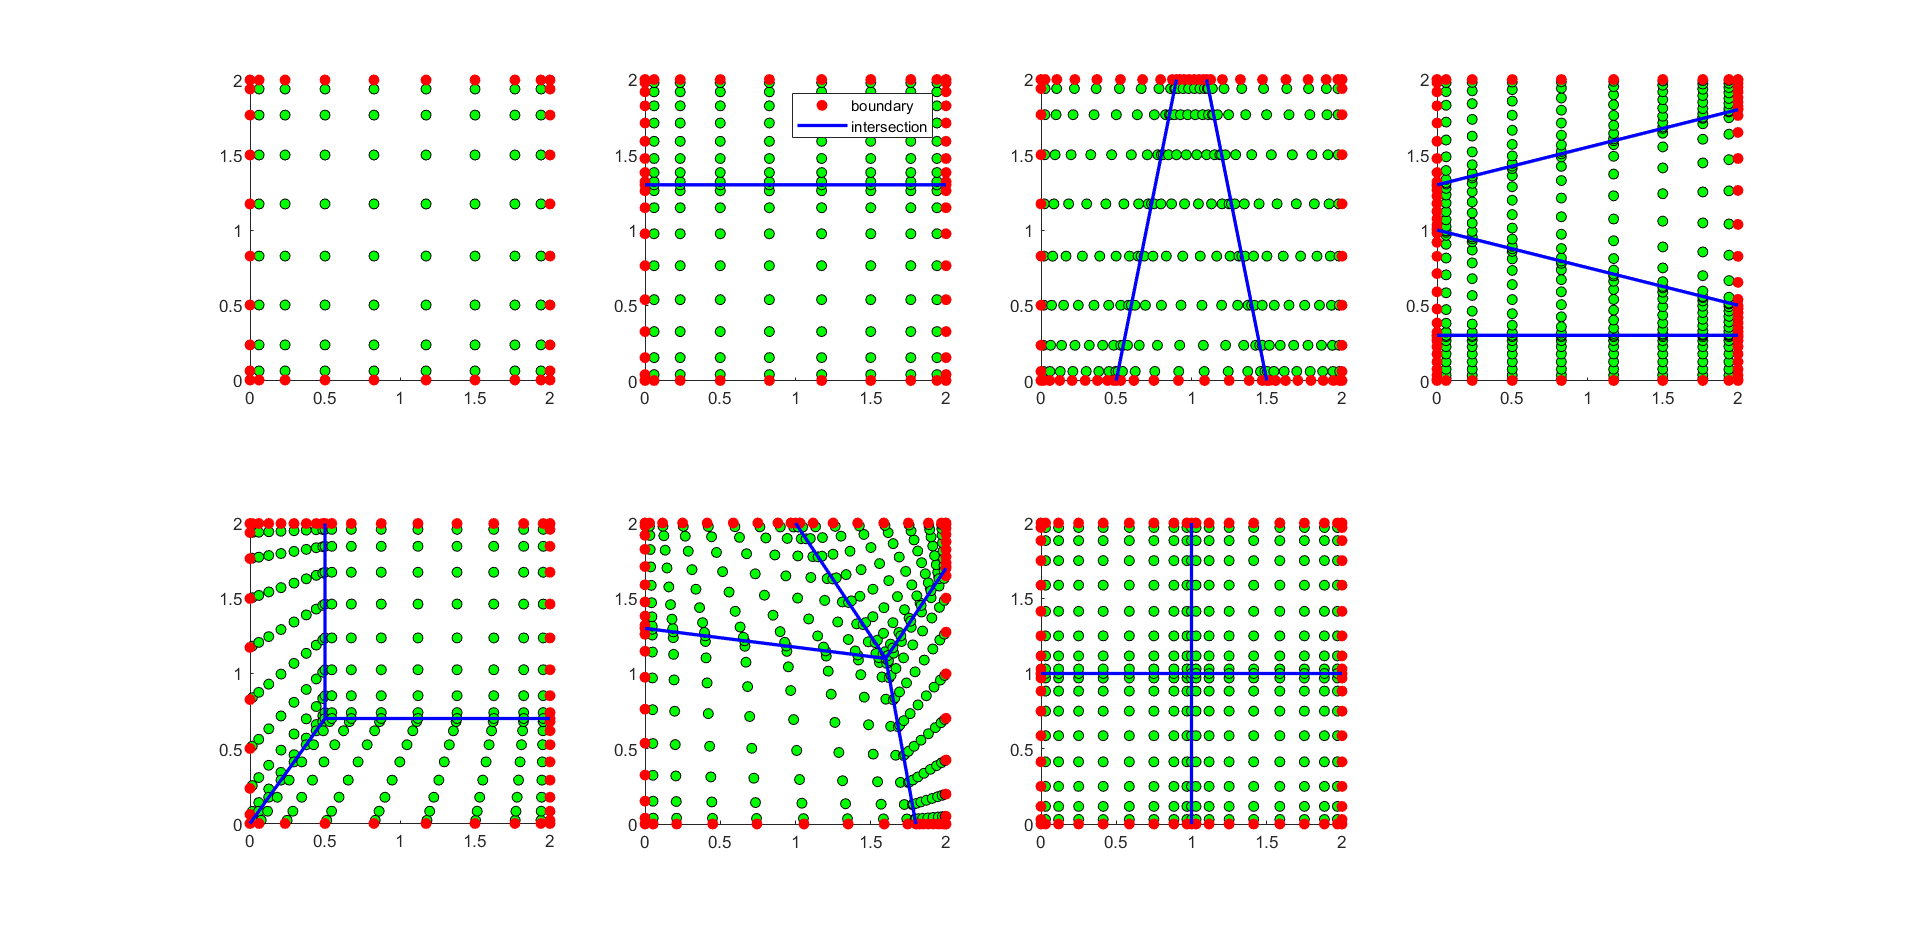
\includegraphics[scale=0.35]{BoxSections.png}
		\caption{Different discretizations of the box (a - g).} 
		\label{F2}
	\end{figure}
	\begin{figure}[h]
		\centering
		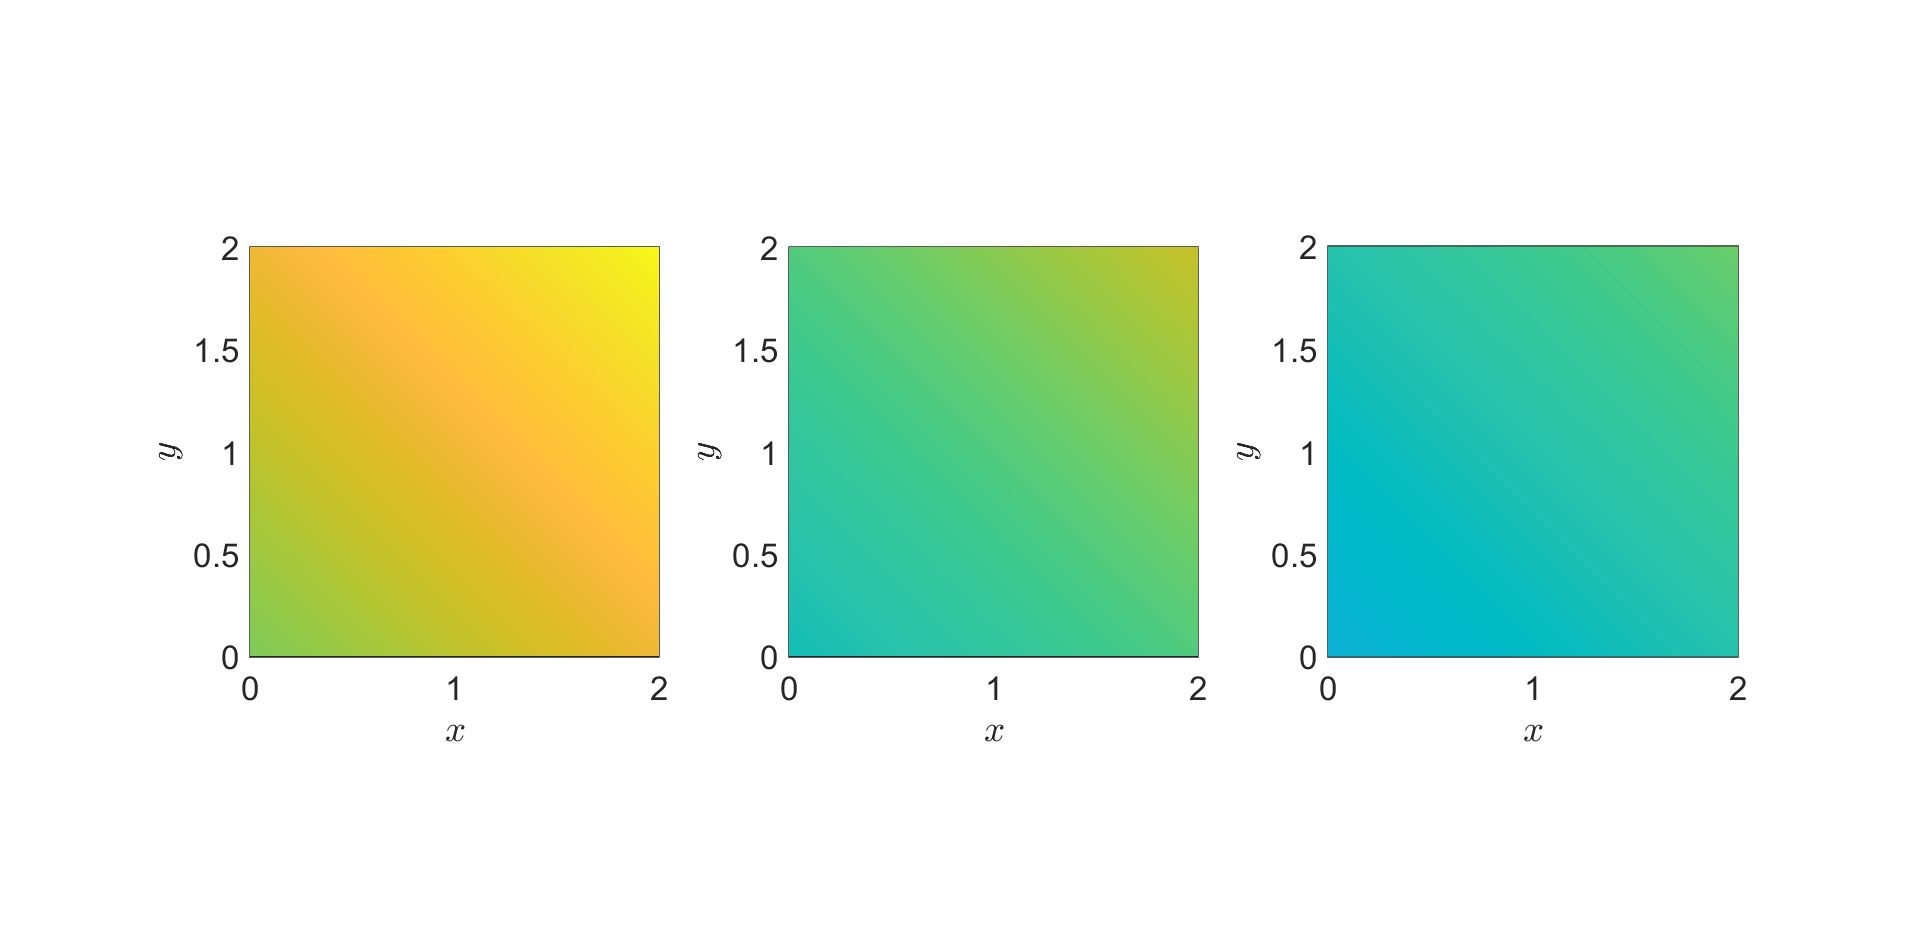
\includegraphics[scale=0.35]{boxEx.png}
		\caption{Exact solution on the box.} 
		\label{F3}
	\end{figure}
	\begin{figure}[h]
		\centering
		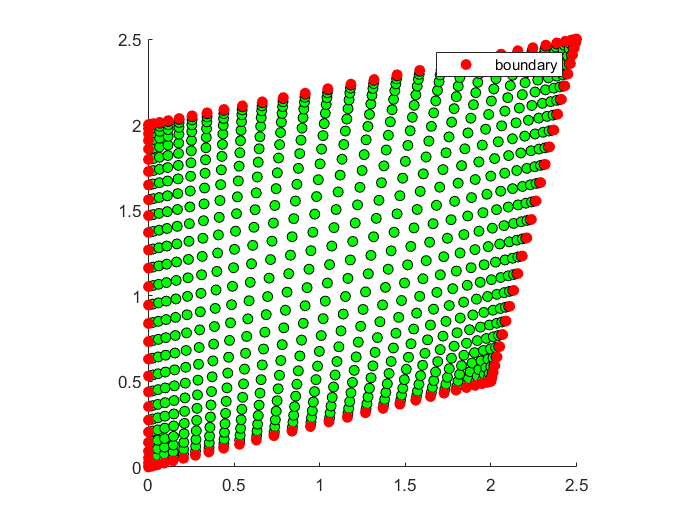
\includegraphics[scale=0.35]{quad.png}
		\caption{Quadrilateral domain (q).} 
		\label{F3a}
	\end{figure}

The same test can be done for a wedge. Here, a single wedge and discretized versions are considered, see Figure \ref{F4}. Table \ref{Tab2:ErrorsExWedge} shows the errors measured against the exact solution for different discretizations of the wedge for $N = 20$ and $N = 30$. The solution can be seen in Figure \ref{F5}.
\begin{figure}[h]
	\centering
	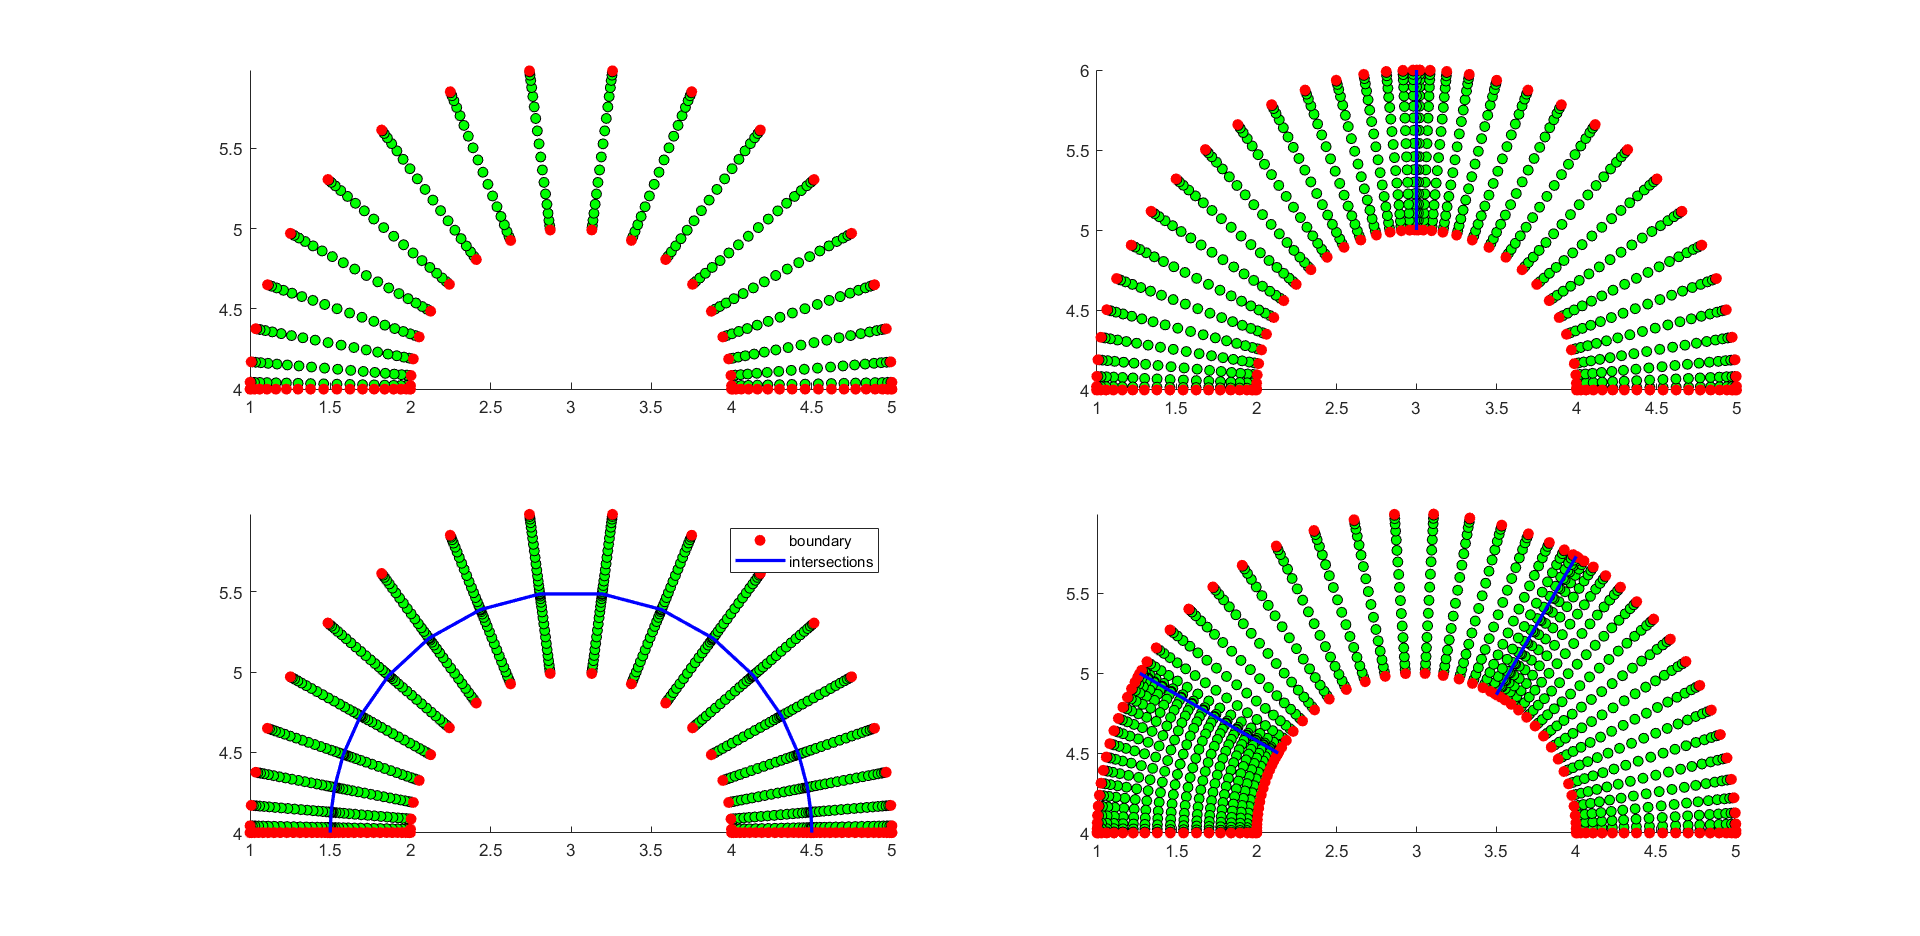
\includegraphics[scale=0.35]{WedgeSections.png}
	\caption{Different discretizations of the wedge (h -k).} 
	\label{F4}
\end{figure}

\begin{figure}[h]
	\centering
	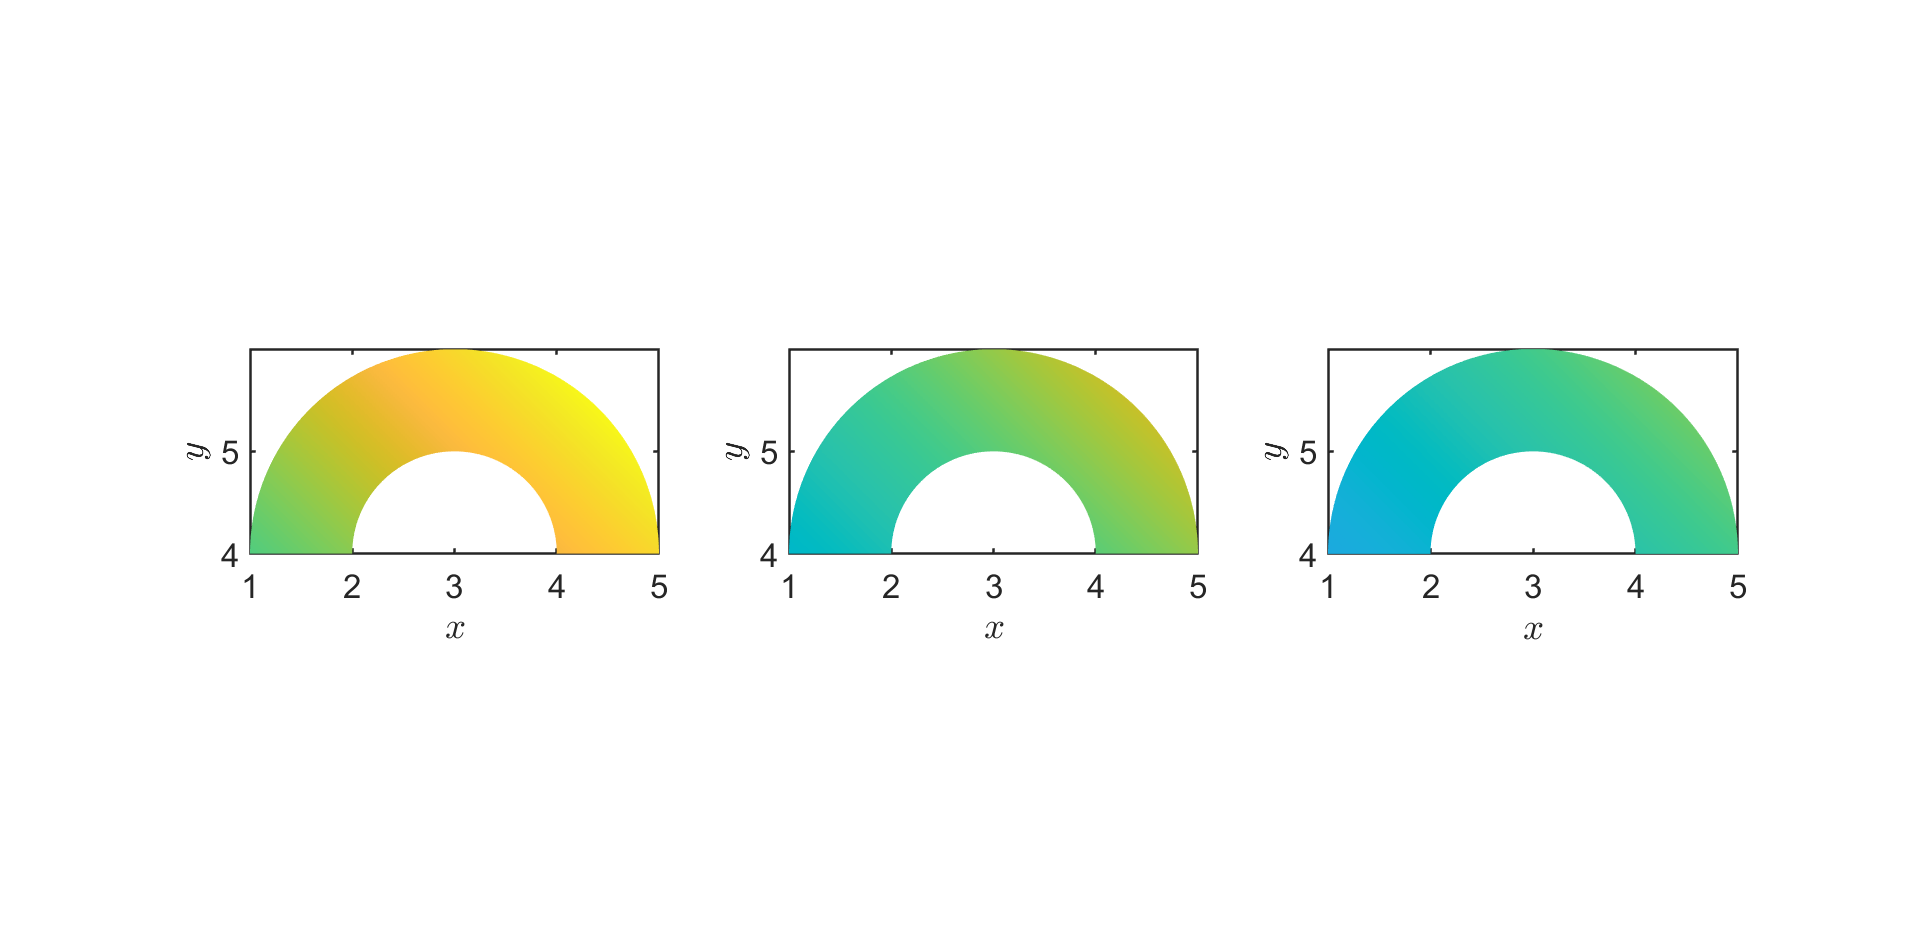
\includegraphics[scale=0.35]{wedgeEx.png}
	\caption{Exact solution on the wedge.} 
	\label{F5}
\end{figure}
\begin{table}
	\caption{Errors compared to exact solution for different discretization (into one, two and three shapes) of the wedge}
	\begin{tabular}{ ||c| c| c| c| c|| }
		\hline
		\hline
		& h & i & j& k\\ 
		\hline
		Abs. Error, $N =10$& $0.0019$ & $3.4678 \times 10^{-6}$ & $0.0026$ & $2.6814\times 10^{-6}$\\  
		Rel. Error, $N =10$& $4.441 \times 10^{-6}$& $6.5183 \times 10^{-9}$ &$4.4489 \times 10^{-6}$ &  $4.0877\times 10^{-9}$\\
		\hline
		Abs. Error, $N =20$& $3.1141 \times 10^{-7}$ & $3.9526 \times 10^{-7}$ & $4.2335\times 10^{-7}$ & $4.4145\times 10^{-7}$\\  
		Rel. Error, $N =20$& $7.4762 \times 10^{-10}$& $7.5984 \times 10^{-10}$ &$7.4942 \times 10^{-10}$ &  $7.0897 \times 10^{-10}$\\
		\hline
		Abs. Error, $N =30$& $ 2.7613\times 10^{-7}$ & $ 3.8484\times 10^{-7}$ & $3.892\times 10^{-7}$ & $4.3211\times 10^{-7}$ \\  
		Rel. Error, $N =30$ & $ 7.5178\times 10^{-10}$& $ 7.4375\times 10^{-10}$ &$7.5061\times 10^{-10}$ & $6.9683\times 10^{-10}$  \\
		\hline
		\hline
	\end{tabular}
	\label{Tab2:ErrorsExWedge}
\end{table}
Next the advection diffusion equation is solved on a multishape which is composed of four quadrilaterals, see Figure \ref{F6}. The absolute error for $N = 20$ on each shape as compared to the exact solution is $6.1246 \times 10^{-7}$ and the relative error is $1.3259 \times 10^{-9}$. 
\begin{figure}[h]
	\centering
	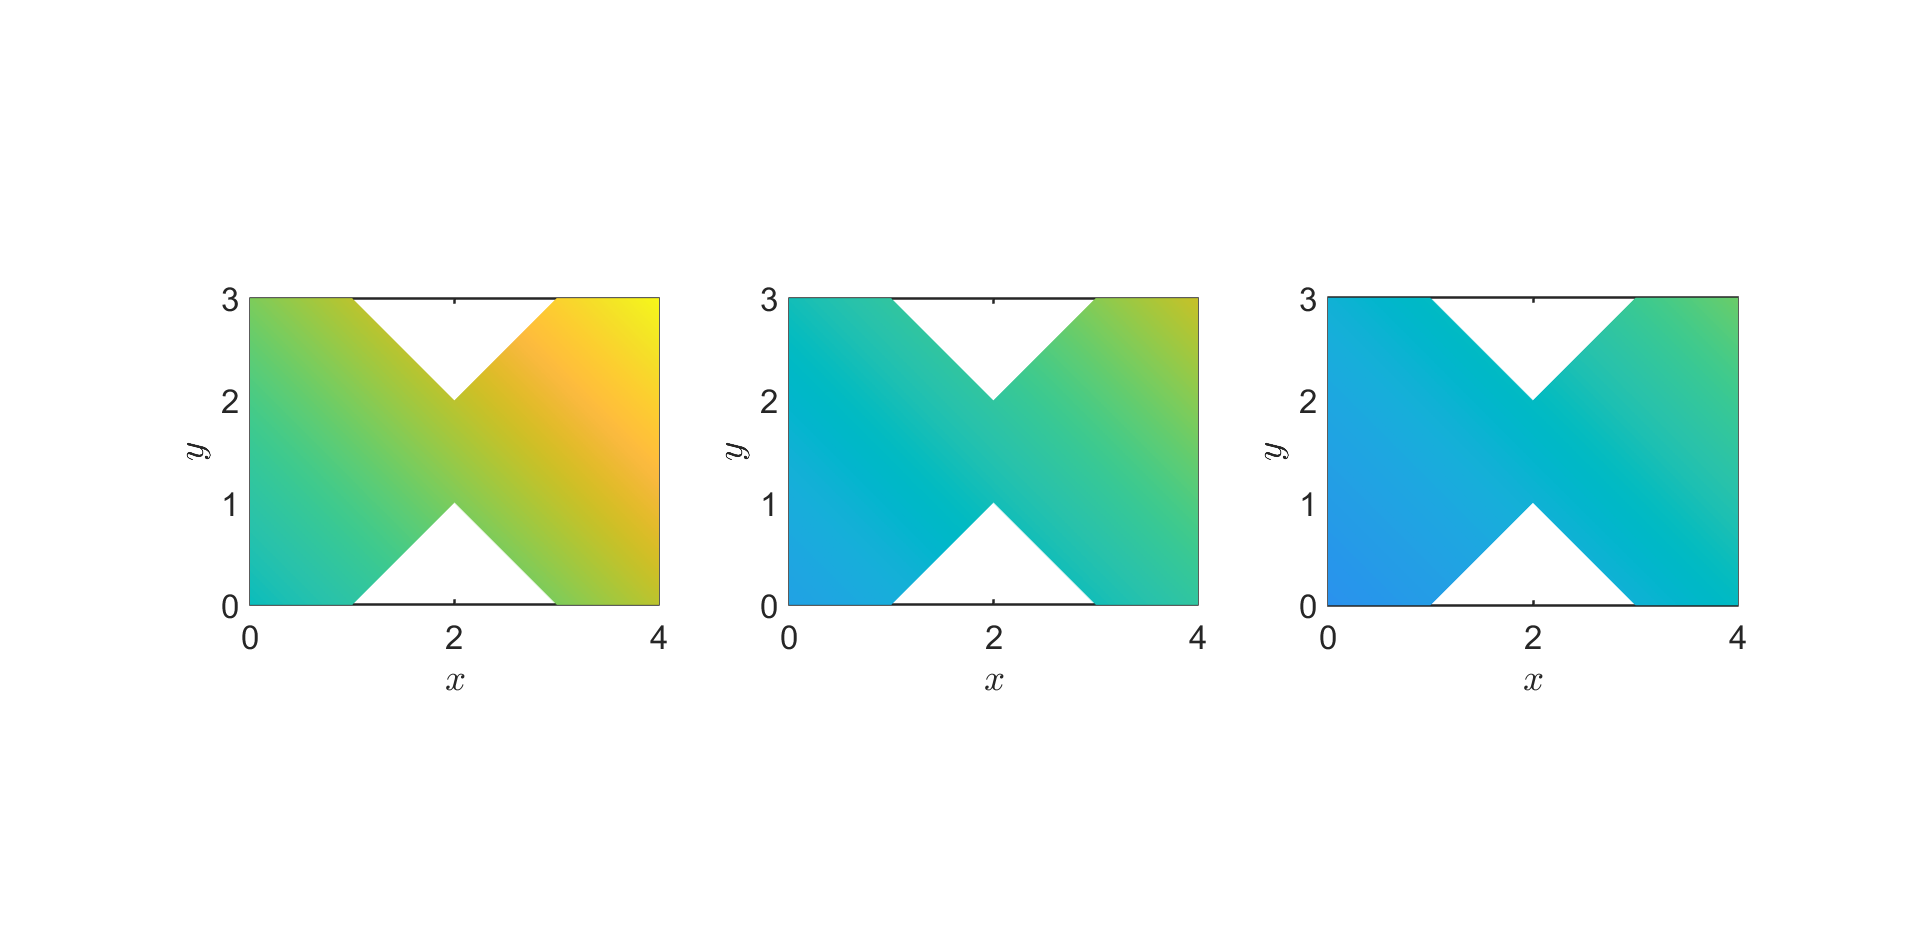
\includegraphics[scale=0.35]{example1.png}
	\caption{Example 1 multishape} 
	\label{F6}
\end{figure}
The same is done for a second example involving a wedge, see Figure \ref{F7}. The absolute error to the exact solution is $3.7239 \times 10^{-7}$ and the relative error is $8.9375 \times 10^{-10}$, when choosing $N= 20$ per shape. 

\begin{figure}[h]
	\centering
	\includegraphics[scale=0.35]{example2.png}
	\caption{Example 2 multishape} 
	\label{F7}
\end{figure}


\subsection{Exact Tests - Dirichlet Conditions, solution 2}

We solve an exact Dirichlet problem which does not have an exponential form but a quadratic form. In order to do this, we add on a source term $f$ to the equation.
We define the exact solution as
\begin{align*}
	\rho &= t y_1^2 y_2^2,\\
	f &= y_1^2 y_2^2 - 2 y_1^2 t - 2 y_2^2 t + 2 y_1 y_2^2 t,
\end{align*}
and with a velocity field of strength one acting in the $y_1$ direction.
We run this on a few of the problems on the box and the wedge (a,b,c,f, h, j, k). The results are displayed in Table \ref{Tab4}.

\begin{table}
	\caption{Errors for discretization of the box and wedge for a quadratic exact Dirichlet solution}
	\begin{tabular}{ ||c| c| c| c| c |c|c|| }
		\hline
		\hline
		& A.E. $N =10$ & R.E. $N =10$ &A.E. $N =20$ & R.E. $N =20$ &A.E. $N =30$ & R.E. $N =30$ \\ 
		\hline
		a & $ 2.2747\times 10^{-13 }$ & $ 3.9799\times 10^{-16 }$ & $ 3.9207\times 10^{-13 }$ & $6.3023 \times 10^{-16 }$ & $4.7291 \times 10^{- 13}$ & $ 7.5978\times 10^{-16 }$\\  
		b & $ 1.1317\times 10^{-12 }$ & $1.1097 \times 10^{-15}$ & $6.1443 \times 10^{-13 }$ & $ 5.985\times 10^{-16 }$ & $2.5646 \times 10^{- 12}$ & $2.5682 \times 10^{-15 }$\\  
		c & $ 7.0072\times 10^{- 13}$ & $ 7.0033 \times 10^{-16 }$ & $1.4084 \times 10^{-12 }$ & $ 1.3513\times 10^{- 15}$ & $2.0691 \times 10^{- 12}$ & $ 2.4102\times 10^{-15 }$\\  
		f & $ 8.2166\times 10^{- 13}$ & $1.6362\times 10^{- 15} $ & $ 1.5548 \times 10^{-12 } $ & $1.0522 \times 10^{-15 }$ & $2.6986 \times 10^{-12} $ & $ 1.7149\times 10^{- 15}$\\  
	    \hline
		h & $0.0262 $ & $3.1608 \times 10^{-7}$ & $ 5.9536\times 10^{- 11}$ & $7.4829 \times 10^{-16 }$ & $ 8.2469\times 10^{-11}$ & $ 1.0421\times 10^{-15}$\\  
		j & $13.0821 $ & $0.0002 $ & $ 5.1279 \times 10^{- 6}$ & $6.1963 \times 10^{-11 }$ & $2.1582 \times 10^{- 10}$ & $ 2.7077\times 10^{-15}$\\  
		k & $0.0193$ & $ 2.0145\times 10^{- 7}$ & $6.8171 \times 10^{-11 }$ & $ 7.4486\times 10^{-16 }$ & $ 9.9529 \times 10^{-11}$ & $ 1.0842\times 10^{-15}$\\  
		\hline
		\hline
	\end{tabular}
	\label{Tab4}
\end{table}

\subsection{Exact Tests - No-Flux Conditions}
We consider an exact solution on a box with no-flux boundary conditions for the advection diffusion equation. The solution is
\begin{align*}
	 \rho = 2 + \exp(-(\mu_1^2 + \mu_2^2)t)\cos(\mu_1 y_1)\cos(\mu_2 y_2),
\end{align*}
where $	\mu_1 = n\pi/L_1$, $\mu_2 = n\pi/L_2$ and $n = 2$, $L_1 = d - c$, $ L_2 = b - a$ for a domain $ [a,b]\times [c,d]$. We use the discretizations of the box displayed in Figure \ref{F2}. The exact solution for this problem can be seen in Figure \ref{F3b}.
\begin{figure}[h]
	\centering
	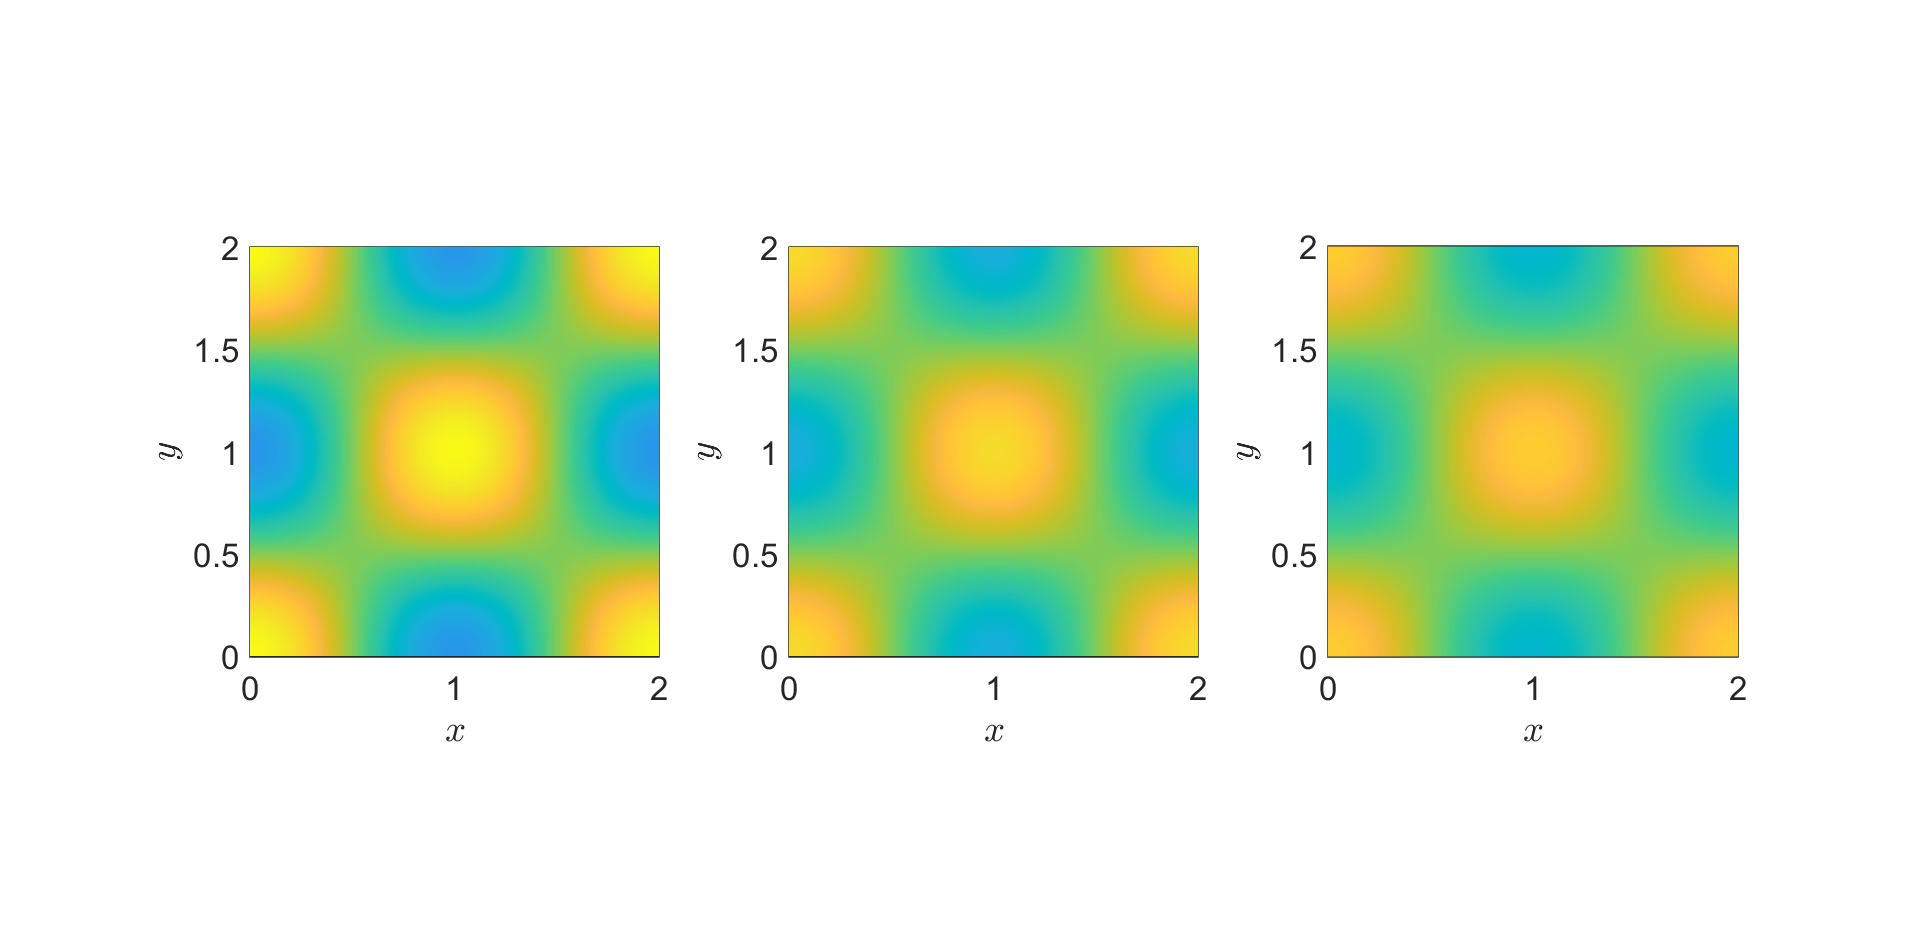
\includegraphics[scale=0.35]{boxExNoFlux.png}
	\caption{Exact solution on the box with no-flux boundary conditions.} 
	\label{F3b}
\end{figure}
\begin{table}
	\caption{Errors compared to exact solution with no-flux boundary conditions for different discretization of the box (absolute error A.E. and relative error R.E. are compared)}
	\begin{tabular}{ ||c| c| c| c| c |c|c|| }
		\hline
		\hline
		& A.E. $N =10$ & R.E. $N =10$ &A.E. $N =20$ & R.E. $N =20$ &A.E. $N =30$ & R.E. $N =30$ \\ 
		\hline
		a & $0.0105$ & $2.523 \times 10^{-5}$ & $2.8349\times 10^{-7}$ & $6.862\times 10^{-10}$ & $2.682\times 10^{-7}$ & $6.4921\times 10^{-10}$\\  
		b & $0.0102$ & $1.7387\times 10^{-5}$ & $3.5488\times 10^{-7}$ & $6.0816\times 10^{-10}$ & $3.5538\times 10^{-7}$ & $6.0901\times 10^{-10}$\\  
		c & $0.0713$ & $9.8994 \times 10^{-5}$ & $0.0070$ & $9.7842\times 10^{-6}$ & $0.0026$ & $3.6463\times 10^{-6}$\\  
		d & $0.0849$ & $0.0001               $ & $0.0083$ & $9.9356\times 10^{-6}$ & $0.0030$ & $3.6506\times 10^{-6}$\\  
		e & $0.0057$ & $8.1264 \times 10^{-6}$ & $4.3058\times 10^{-7}$ & $6.0667\times 10^{-10}$ & $4.3145\times 10^{-7}$ & $6.0789\times 10^{-10}$\\  
		f & $0.1293$ & $0.0002$ & $0.0135$ & $1.6099\times 10^{-5}$ & $0.0040$ & $4.8753\times 10^{-6}$\\  
		g & $8.7462 \times 10^{-6}$ & $1.0753\times 10^{-8}$ & $5.1503\times 10^{-7}$ & $6.2334\times 10^{-10}$ & $5.147\times 10^{-7}$ & $6.2295\times 10^{-10}$\\  
		\hline
		\hline
	\end{tabular}
	\label{Tab3:ErrorsNoFlux}
\end{table}




\section{Forward Problems on multishapes}
We first consider a forward problem on the different discretizations of the box, see Figure \ref{F2}. We compare the results of the discretized boxes with the result for box (a) with large $N$.
We choose the initial condition for $\rho$ to be
\begin{align*}
	\rho_0 = \exp(-2((y_1 - 0.7 )^2 + (y_2 - 0.2)^2))
\end{align*}
and impose a constant flow of strength $0.8$ acting upward.
We choose $N = 20$ and $N = 30$ as before. The errors are displayed in Table \ref{Tab3:ErrorsFWBox} and the result can be seen in Figure \ref{FFW1}. 

\begin{table}
	\caption{Errors (compared to whole box with $N = 50$) for different discretizations of the box}
	\begin{tabular}{ ||c| c| c| c| c| c| c|| }
		\hline
		\hline
		& b & c & d & e & f & g\\ 
		\hline
		Abs. Error, $N =20$& $0.0129$ & $0.0194$ & $0.0337$& $0.032$&  $ 0.0165$ & $0.0099$ \\  
		Rel. Error, $N =20$& $0.001$& $0.0025$ & $0.0024$ & $0.0025$& $0.0019$  & $0.0007$ \\
		Abs. Error, $N =30$& $0.0054$ & $0.0078$ & $0.0137$ &$0.0134$&$0.0064$& $0.0026$\\  
		Rel. Error, $N =30$ & $0.0003$& $0.0007$ &$0.0006$ &$0.0007$&$0.0005$& $0.0001$\\
		\hline
		\hline
	\end{tabular}
	\label{Tab3:ErrorsFWBox}
\end{table}
\begin{figure}[h]
	\centering
	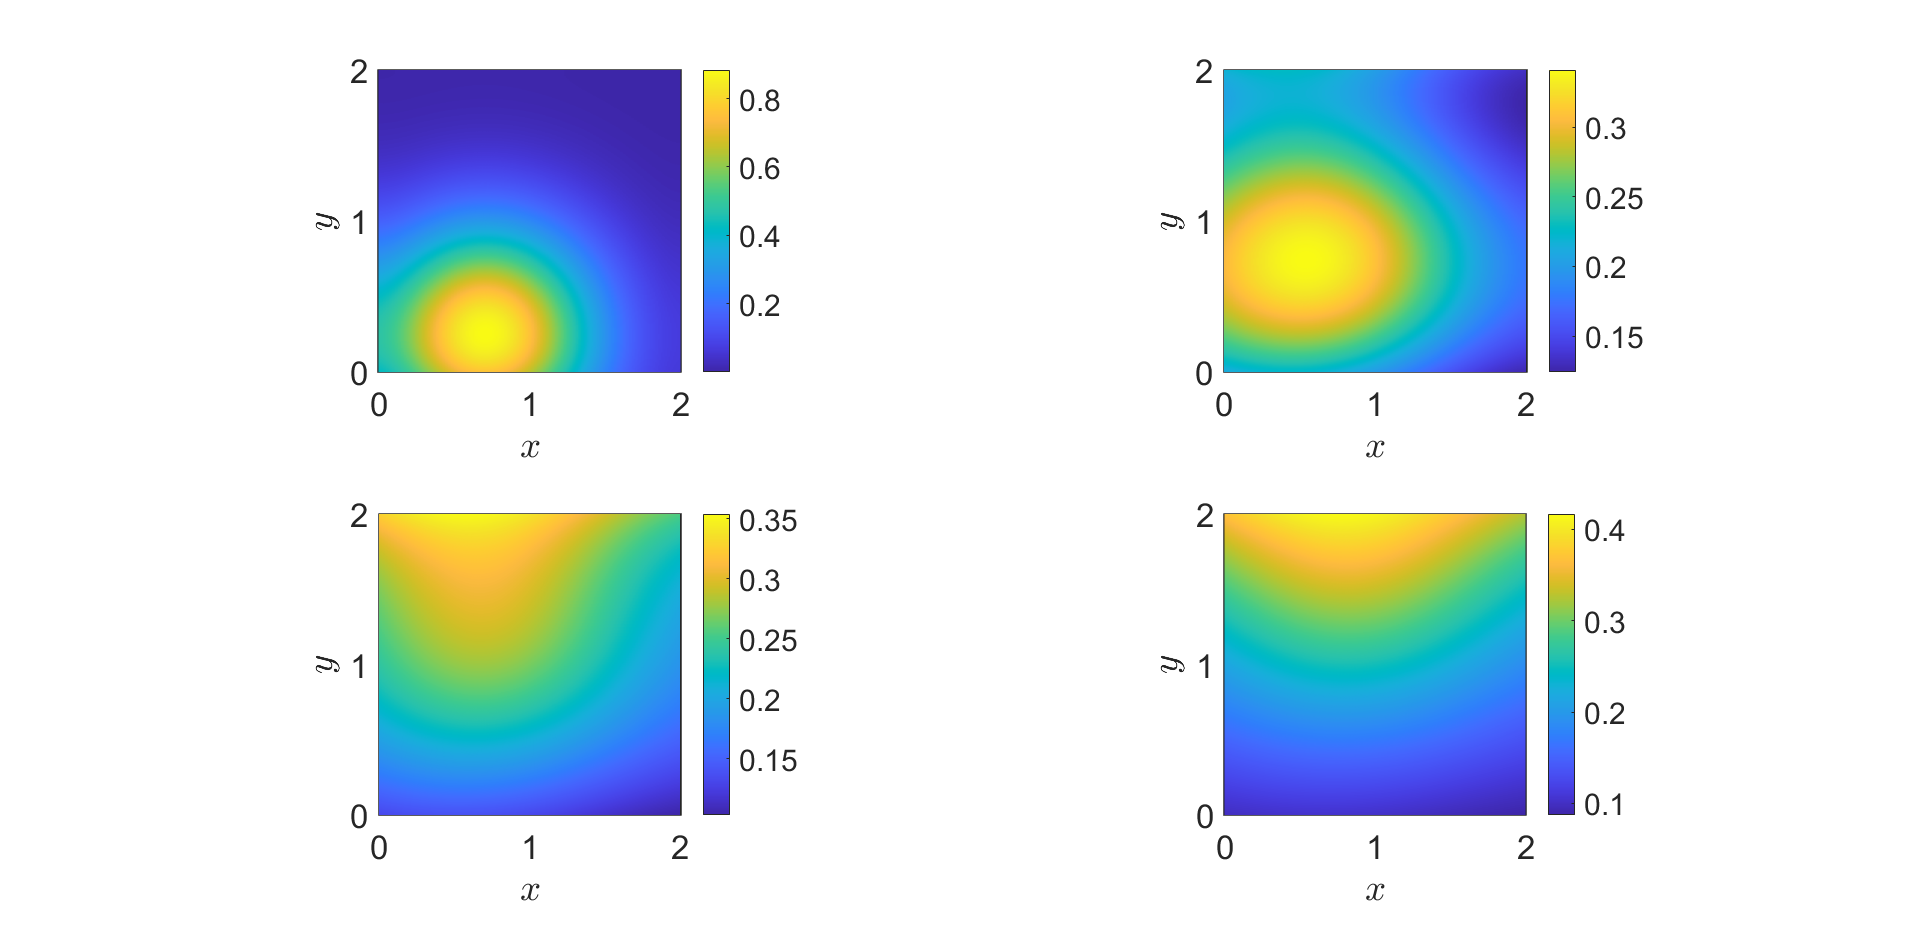
\includegraphics[scale=0.35]{FWBox.png}
	\caption{Forward Example on box discretizations} 
	\label{FFW1}
\end{figure}


We follow the same idea, but now consider the wedge discretizations, see Figure \ref{F4}. We choose the initial condition for $\rho$ to be
\begin{align*}
	\rho_0 = \exp(-2((y_1 - 1.5 )^2 + (y_2 - 4.5)^2))
\end{align*}
and impose a constant flow of strength $3$ acting from left to right, along the angular direction.
We choose $N = 20$ and $N = 30$. The errors are displayed in Table \ref{Tab4:ErrorsFWWedge} and the result can be seen in Figure \ref{FFW2}. 

\begin{table}
	\caption{Errors (compared to whole wedge (h) ) for different discretization (into two and three shapes) of the wedge}
	\begin{tabular}{ ||c| c| c| c|| }
		\hline
		\hline
		& i & j &k\\ 
		\hline
		Abs. Error, $N =20$& $0.0233 $ & $0.0750 $ & $0.0189 $ \\  
		Rel. Error, $N =20$& $0.0026 $& $0.0068 $ &$0.0013 $ \\
		Abs. Error, $N =30$& $0.0071 $ & $0.0316 $ & $0.0113 $  \\  
		Rel. Error, $N =30$ & $0.0005 $& $0.0019 $ &$ 0.0005$  \\
		\hline
		\hline
	\end{tabular}
	\label{Tab4:ErrorsFWWedge}
\end{table}
\begin{figure}[h]
	\centering
	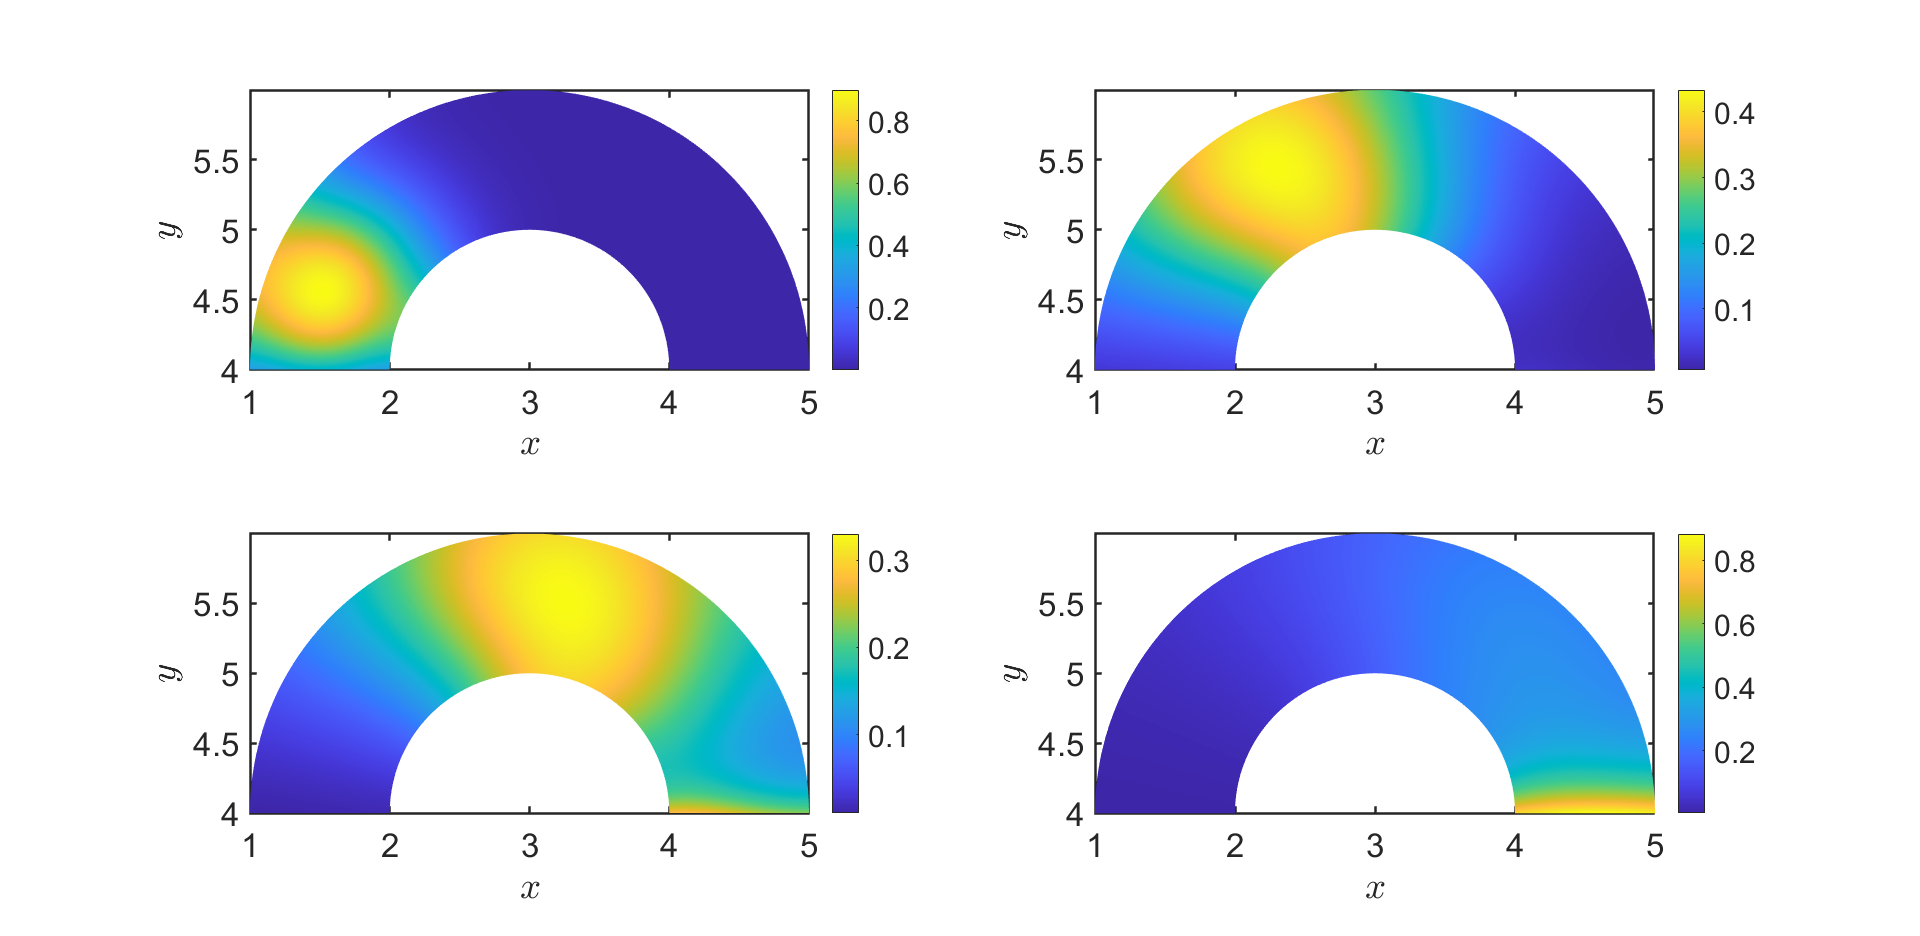
\includegraphics[scale=0.35]{FWWedge.png}
	\caption{Forward Example on wedge discretizations} 
	\label{FFW2}
\end{figure}



Finally, two multishape examples are shown, which are of interesting shapes.
The first of these examples is solving an advection diffusion problem on a multishape consisting of two quadrilaterals and two wedges, with constant velocity of strength ten. The initial condition for this problem is:
 \begin{align*}
 	\rho_0 = \exp( -2(y_1 -0.5)^2 - 2 (y_2 + 1)^2).
 \end{align*}
The result, evaluated for $N= 20$ on each shape, can be seen in Figure \ref{F8}.

\begin{figure}[h]
	\centering
	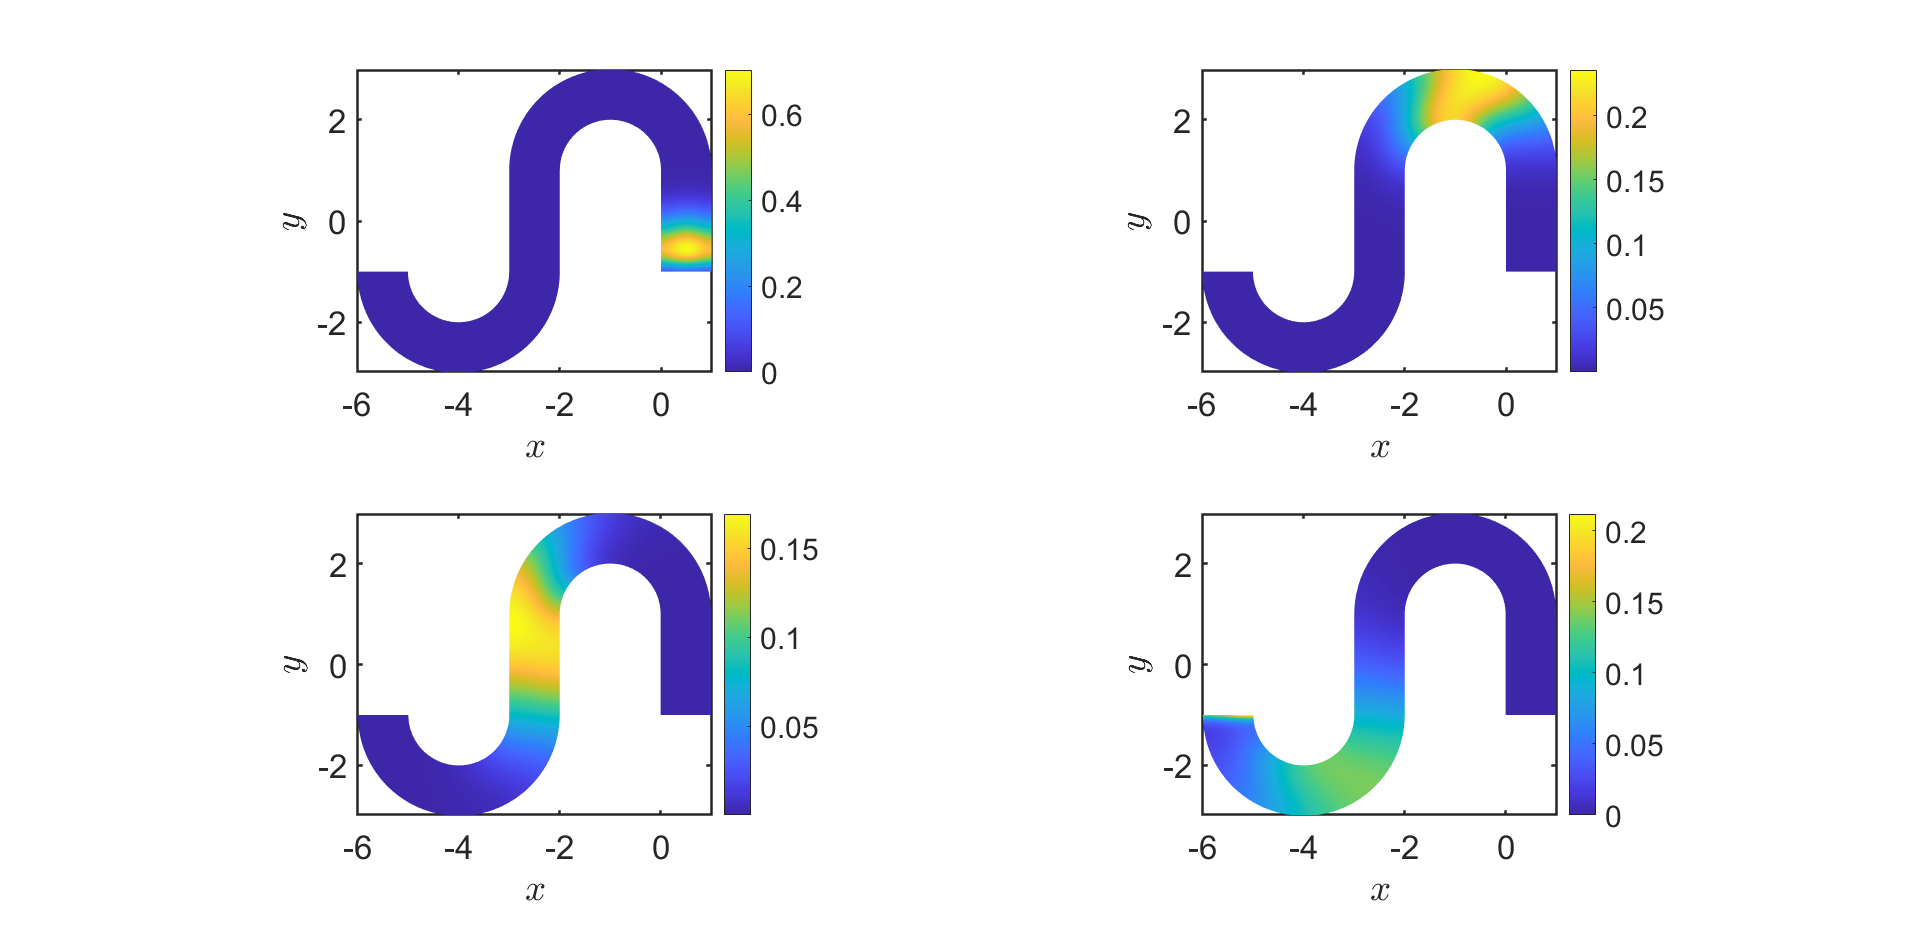
\includegraphics[scale=0.35]{ex1.png}
	\caption{Forward Problem 1, different colour scale for each plot to highlight particle mass location}
	\label{F8}
\end{figure}

In a second example, the velocity is of strength $5$ and the initial condition is:
 \begin{align*}
	\rho_0 = \exp( -2(y_1 -0.5)^2 - 2 (y_2 - 1.5)^2).
\end{align*}
The result, which is computed on a multishape made up of four quadrilaterals into a channel, can be seen in Figure \ref{F9}.

\begin{figure}[h]
	\centering
	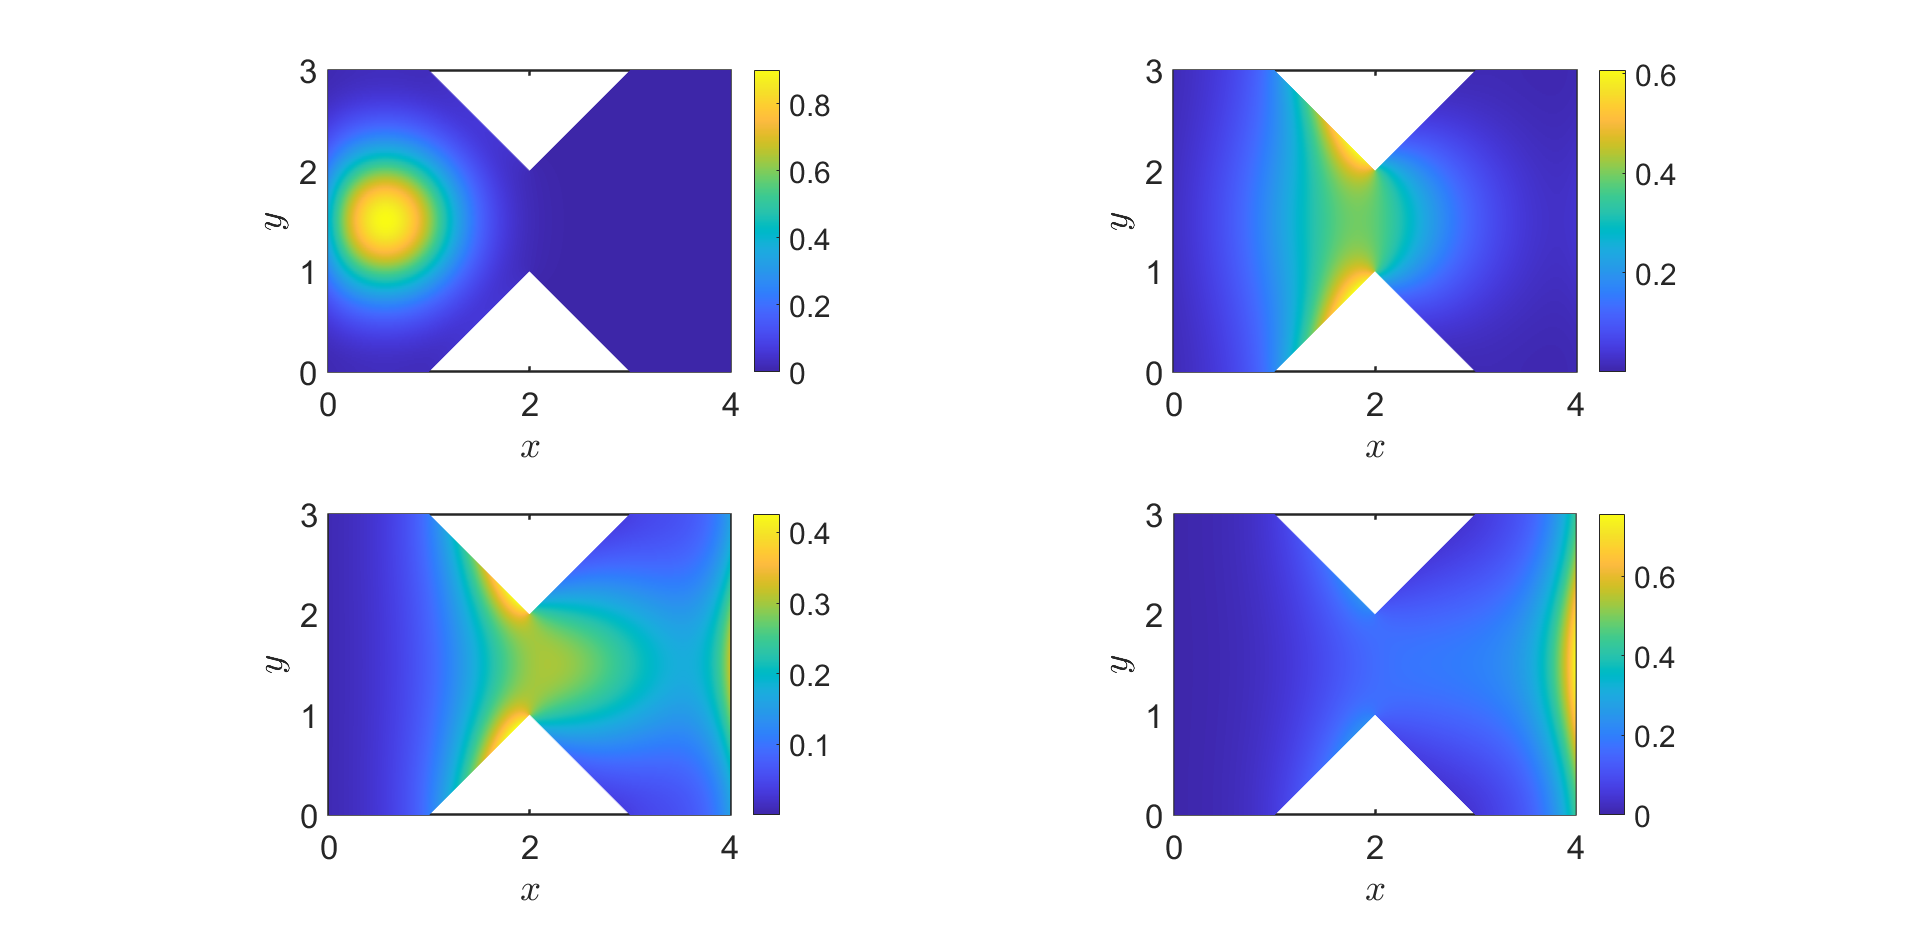
\includegraphics[scale=0.35]{ex2.png}
	\caption{Forward Problem 2, different colour scale for each plot to highlight particle mass location}
	\label{F9}
\end{figure}








\pagebreak	
\bibliography{GeneralBib}
\bibliographystyle{unsrt}
\end{document}